\section{Introdução}

Sabões são produtos muitos utilizados no dia a dia de muitas pessoas por todo o planeta, eles podem 
vir várias formas barras, flocos, grânulos, soluções. Porém, independente de seu formato, estado físico
ou textura todo sabão de produzido usando o mesmo mecanismo. A saponificação é uma reação que transforma
gorduras e óleos em sabões de diversos tipos.

O principal uso do sabão é na higienização de locais, superfícies e do próprio corpo, função essa
possibilitada pela sua capacidade de remover gorduras e sujidades em meio aquoso. Essa propriedade é 
diretamente determinada pela estrutura química da molécula do sabão, ilustrada na Figura~\ref{fig:estrutura_sabao}. 
Tal molécula é composta por uma longa cadeia carbônica apolar e uma extremidade polar, geralmente
um carboxilato. Essa natureza anfifílica permite que o sabão atue simultaneamente em meios polares
e apolares: a porção lipofílica interage com óleos e gorduras, enquanto a extremidade hidrofílica se
dissolve em água. Em solução aquosa, as moléculas de sabão se organizam espontaneamente em estruturas
denominadas micelas, nas quais as cadeias apolares ficam voltadas para o interior, encapsulando as 
partículas de gordura, e as extremidades polares permanecem em contato com a água, viabilizando a
dispersão e a remoção das sujidades.

\begin{figure}[H]
    \centering
    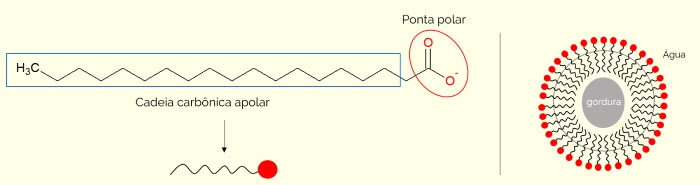
\includegraphics[width=0.7\textwidth]{src/fig/estrutura_sabao.jpg}
    \caption{Estrutura molecular do sabão e de suas micelas \cite{santos2021saponificacao}}
    \label{fig:estrutura_sabao}
\end{figure}

Na saponificação, o óleo vegetal utilizado como matéria-prima não é apenas um simples reagente: a composição 
de seus ácidos graxos determina diretamente as propriedades físicas e funcionais do produto final \cite{warra2010cold}. 
Óleos ricos em ácidos graxos saturados de cadeia média, como o óleo de babaçu, tendem a gerar sabões 
mais duros e com maior formação de espuma, enquanto óleos com alto teor de ácidos graxos insaturados 
de cadeia longa, como o óleo de soja, resultam em barras mais macias e com menor poder de limpeza. 
%Essa diferença se deve ao grau de empacotamento molecular dos sais de ácidos graxos formados: cadeias 
%saturadas se organizam de forma mais compacta e ordenada na matriz sólida, conferindo maior rigidez 
%estrutural ao sabão.

Diante disso, a utilização de misturas de óleos surge como estratégia para combinar as propriedades 
desejáveis de diferentes matérias-primas, permitindo o ajuste fino das características do produto \cite{silva2021producao}. 
A proporção entre óleos de perfis distintos — como um óleo láurico e um óleo rico em insaturações — 
define um balanço entre dureza, formação de espuma e poder de limpeza, tornando a formulação da mistura 
uma variável crítica no desenvolvimento do sabão. Além disso, o aproveitamento de óleos residuais de 
fritura nessa composição representa uma alternativa alinhada aos princípios da Química Verde, transformando 
um resíduo de grande geração na indústria alimentícia em produto de valor agregado \cite{castro2020producao}.
